% !TEX encoding = UTF-8 Unicode
% !TEX TS-program = pdflatex

% toptesti document class
\documentclass[%
    a4paper, % not needed, by default it is a4paper, or also b5paper can be used
    corpo=12pt, % dimension of basic font
    % oneside is generally the way to go
    oneside, % two side optimizes for two-face printing, having chapters open on the right (aka odd numbers), if you don't want blank pages put oneside here
    stile=standard,
    %evenboxes, % not needed, to put supervisors and candidate at the same level
    tipotesi=magistrale,
    numerazioneromana, % roman numbering for appendixes and preambles, up to Table of Contents
    openright, % to force opening on the right for double-sided printing
    cucitura=7mm, % for printing, 7mm should be enough
    %dvipsnames, % for compatibility with xcolor, it does not work
]{toptesi}

%%%%%%%%%%%%%%%%%%%%%%%%%%%%%%%%%%%%%%%%%%%%%%%%%%%%
\usepackage[english]{babel}
\usepackage[utf8]{inputenc}
\usepackage[T1]{fontenc}
\usepackage{lmodern}

\usepackage{hyperref} % must be loaded before glossaries-extra

% bibliography
\usepackage[hyperref=true,backref=true,backend=biber,maxbibnames=9,maxcitenames=2,style=numeric,citestyle=numeric,sorting=none]{biblatex} % hyperref uses links, backref goes back to citations, uses biber as backend, with 9 names at most in bibliography and 2 in citations, citing using numbers, and sorting in citation order
% sorting can be also ydnt for year descending, name, title or ynt for ascending year

\usepackage{adjustbox} % to resize boxes by keeping the same aspect ratio
\usepackage{algorithm} % algorithm environment
\usepackage{algpseudocode} % improved pseudo-code
\usepackage{amsfonts}               %  AMS mathematical fonts
\usepackage{amsmath}
\usepackage{amssymb}                %  AMS mathematical symbols
\usepackage{bm}                     %  black/bold mathematical symbols
\usepackage{booktabs}               %  better tables
\usepackage[labelfont=bf]{caption} % font=footnotesize % to have reduced caption font size
\usepackage{csquotes}
\usepackage{enumitem} %left align the bulleted points
\usepackage{geometry}
%\usepackage{glossaries} % to use acronyms and glossary, it has also glossaries-extra as extension, but commands are different
\usepackage[%
    toc, % puts the link in the ToC
    %record, % to use bib2gls
    abbreviations, % to load abbreviations / acronyms
    nonumberlist, % to avoid printing the numbers of the references in the acronyms page
]{glossaries-extra}
\usepackage{graphicx}               %  post-script images
%\usepackage{iwona} % extra fonts, substitute standard ones
\usepackage{listings} % to insert formatted code
\usepackage{lipsum} % for lorem ipsum text, not needed in the real work
\usepackage{makecell} % to change dimensions of cells, for math cases
\usepackage{mathtools} % for additional commands
\usepackage{mfirstuc} % to have capitalization capabilities
\usepackage[final]{microtype}      % microtypography, final lets latex use it also in bibliography
\usepackage{multirow} % to allow for cells covering more than 1 row in tables
\usepackage{nicefrac}       % compact symbols for 1/2, etc.
%\usepackage[lofdepth,lotdepth]{subfig}
\usepackage{ragged2e} % for justifying text
\usepackage{siunitx} % support for SI units of measurement and number typesetting
\usepackage{subfig}
\usepackage{svg} % for svg support, works only if inkscape is installed, default for Overleaf v2
%\usepackage{subfigure}              %  subfigure compatibility, can be removed if subfig
\usepackage{tabularx} % equal-width columns in tables
\usepackage{textcomp} % extra fonts and symbols
\usepackage{url}            % simple URL typesetting
\usepackage{verbatim} % for extended verbatim support
\usepackage{xcolor} % to define colors and use standard CSS names add dvipsnames as option, but it clashes with xcolor loaded in toptesi, pay attention that if it goes in conflict with tikz/beamer, simply use \documentclass[usenames,dvipsnames]{beamer}, along with other custom options when defining the document class


% configuration for glossaries
% convert and load converted glossaries in .tex ,format from .bib
\setabbreviationstyle{long-short-desc} % style before loading resources
% this command sets the style to title for long names of acronyms only in the glossary description, leading to capitalized first-letter for all words
% \glssetcategoryattribute{\glsxtrabbrvtype}{glossname}{capitalisewords} % doesn't work
% resources to load if using a bib file with bib2gls
%\GlsXtrLoadResources[%
% src={glossaries}, % name of the file without extension
% selection=all, % select all the entries
%]
% not needed
%\newglossary*{abbreviation}{Acronyms} % to change the name of this glossary for acronyms

%\renewcommand{\glsclearpage}{\paginavuota} % to allow glossaries to clear pages, done manually is better

% setup for verbatim
\makeatletter
\def\verbatim@font{\footnotesize\ttfamily}
\makeatother


% setup for hyperref
\hypersetup{%
    pdfpagemode={UseOutlines},
    bookmarksopen,
    pdfstartview={FitH},
    colorlinks,
    linkcolor={black}, % it is suggested to keep them black, since when printing it it costs per page, and if they have color it's twice the price per page
    citecolor={black},
    urlcolor={black}
  }
%

% setup for svg
\svgsetup{%
    inkscapeformat=pdf, % to force usage of PDF
    inkscapelatex=false, % to disable latex rendering of text, produces errors
}

% setup for siunitx, it does not work in the summary
\sisetup{%
    detect-all, % to use the same font as for writing when using \num
    mode=text, % to allow it to work also in math mode
    group-separator = {,}, % separator for number grouping
    group-minimum-digits = 3, % minimum number of digits a number must have to be grouped in 3-digit groups
}

% listings colours
\definecolor{rulecolor}{rgb}{0,0,0}
\definecolor{commentcolor}{rgb}{0,0.6,0}
\definecolor{linenumbercolor}{rgb}{0.5,0.5,0.5}
\definecolor{keywordcolor}{rgb}{0,0,0.95}
\definecolor{backcolor}{rgb}{1,1,1}%{0.95,0.95,0.92}
\definecolor{stringcolor}{rgb}{0.58,0,0.82}

% setup for lstlisting
\lstset{ %
	backgroundcolor=\color{backcolor},   % choose the background color; you must add \usepackage{color} or \usepackage{xcolor}; should come as last argument
	basicstyle=\ttfamily\footnotesize,        % the size of the fonts that are used for the code
	breakatwhitespace=false,         % sets if automatic breaks should only happen at whitespace
	breaklines=true,                 % sets automatic line breaking
	captionpos=t,                    % sets the caption-position to bottom
	commentstyle=\color{commentcolor},    % comment style
	extendedchars=true,              % lets you use non-ASCII characters; for 8-bits encodings only, does not work with UTF-8
	frame=single,	                   % adds a frame around the code
	keepspaces=true,                 % keeps spaces in text, useful for keeping indentation of code (possibly needs columns=flexible)
	keywordstyle=\color{keywordcolor},       % keyword style
	%language=VHDL,                 % the language of the code
	numbers=left,                    % where to put the line-numbers; possible values are (none, left, right)
	numbersep=5pt,                   % how far the line-numbers are from the code
	numberstyle=\tiny\color{linenumbercolor}, % the style that is used for the line-numbers
	rulecolor=\color{rulecolor},         % if not set, the frame-color may be changed on line-breaks within not-black text (e.g. comments (green here))
	showspaces=false,                % show spaces everywhere adding particular underscores; it overrides 'showstringspaces'
	showstringspaces=false,          % underline spaces within strings only
	showtabs=false,                  % show tabs within strings adding particular underscores
	stepnumber=1,                    % the step between two line-numbers. If it's 1, each line will be numbered
	stringstyle=\color{stringcolor},     % string literal style
	tabsize=4,	                   % sets default tabsize to 2 spaces
	title=\lstname,                   % show the filename of files included with \lstinputlisting; also try caption instead of title
	inputencoding=utf8,
	literate=
	{á}{{\'a}}1 {é}{{\'e}}1 {í}{{\'i}}1 {ó}{{\'o}}1 {ú}{{\'u}}1
	{Á}{{\'A}}1 {É}{{\'E}}1 {Í}{{\'I}}1 {Ó}{{\'O}}1 {Ú}{{\'U}}1
	{à}{{\`a}}1 {è}{{\`e}}1 {ì}{{\`i}}1 {ò}{{\`o}}1 {ù}{{\`u}}1
	{À}{{\`A}}1 {È}{{\'E}}1 {Ì}{{\`I}}1 {Ò}{{\`O}}1 {Ù}{{\`U}}1
	{ä}{{\"a}}1 {ë}{{\"e}}1 {ï}{{\"i}}1 {ö}{{\"o}}1 {ü}{{\"u}}1
	{Ä}{{\"A}}1 {Ë}{{\"E}}1 {Ï}{{\"I}}1 {Ö}{{\"O}}1 {Ü}{{\"U}}1
	{â}{{\^a}}1 {ê}{{\^e}}1 {î}{{\^i}}1 {ô}{{\^o}}1 {û}{{\^u}}1
	{Â}{{\^A}}1 {Ê}{{\^E}}1 {Î}{{\^I}}1 {Ô}{{\^O}}1 {Û}{{\^U}}1
	{œ}{{\oe}}1 {Œ}{{\OE}}1 {æ}{{\ae}}1 {Æ}{{\AE}}1 {ß}{{\ss}}1
	{ű}{{\H{u}}}1 {Ű}{{\H{U}}}1 {ő}{{\H{o}}}1 {Ő}{{\H{O}}}1
	{ç}{{\c c}}1 {Ç}{{\c C}}1 {ø}{{\o}}1 {å}{{\r a}}1 {Å}{{\r A}}1
	{€}{{\euro}}1 {£}{{\pounds}}1 {«}{{\guillemotleft}}1
	{»}{{\guillemotright}}1 {ñ}{{\~n}}1 {Ñ}{{\~N}}1 {¿}{{?`}}1
}


% biblatex setup
% generally 9000 is ok, if higher than 10000 it's bad
% If you want to break on URL numbers
\setcounter{biburlnumpenalty}{9000}
% If you want to break on URL lower case letters
\setcounter{biburllcpenalty}{9000}
% If you want to break on URL UPPER CASE letters
\setcounter{biburlucpenalty}{9000}


%% Rust listings

\lstdefinelanguage{Rust}{%
  sensitive%
, morecomment=[l]{//}%
, morecomment=[s]{/*}{*/}%
, moredelim=[s][{\color[rgb]{0,0,0.75}}]{\#[}{]}%
, morestring=[b]{"}%
, alsodigit={}%
, alsoother={}%
, alsoletter={!}%
%
%
% [1] reserve keywords
% [2] traits
% [3] primitive types
% [4] type and value constructors
% [5] identifier
%
, morekeywords={break, continue, else, for, if, in, loop, match, return, while}  % control flow keywords
, morekeywords={as, const, let, move, mut, ref, static}  % in the context of variables
, morekeywords={dyn, enum, fn, impl, Self, self, struct, trait, type, union, use, where}  % in the context of declarations
, morekeywords={crate, extern, mod, pub, super}  % in the context of modularisation
, morekeywords={unsafe}  % markers
, morekeywords={abstract, alignof, become, box, do, final, macro, offsetof, override, priv, proc, pure, sizeof, typeof, unsized, virtual, yield}  % reserved identifiers
%
% grep 'pub trait [A-Za-z][A-Za-z0-9]*' -r . | sed 's/^.*pub trait \([A-Za-z][A-Za-z0-9]*\).*/\1/g' | sort -u | tr '\n' ',' | sed 's/^\(.*\),$/{\1}\n/g' | sed 's/,/, /g'
, morekeywords=[2]{Add, AddAssign, Any, AsciiExt, AsInner, AsInnerMut, AsMut, AsRawFd, AsRawHandle, AsRawSocket, AsRef, Binary, BitAnd, BitAndAssign, Bitor, BitOr, BitOrAssign, BitXor, BitXorAssign, Borrow, BorrowMut, Boxed, BoxPlace, BufRead, BuildHasher, CastInto, CharExt, Clone, CoerceUnsized, CommandExt, Copy, Debug, DecodableFloat, Default, Deref, DerefMut, DirBuilderExt, DirEntryExt, Display, Div, DivAssign, DoubleEndedIterator, DoubleEndedSearcher, Drop, EnvKey, Eq, Error, ExactSizeIterator, ExitStatusExt, Extend, FileExt, FileTypeExt, Float, Fn, FnBox, FnMut, FnOnce, Freeze, From, FromInner, FromIterator, FromRawFd, FromRawHandle, FromRawSocket, FromStr, FullOps, FusedIterator, Generator, Hash, Hasher, Index, IndexMut, InPlace, Int, Into, IntoCow, IntoInner, IntoIterator, IntoRawFd, IntoRawHandle, IntoRawSocket, IsMinusOne, IsZero, Iterator, JoinHandleExt, LargeInt, LowerExp, LowerHex, MetadataExt, Mul, MulAssign, Neg, Not, Octal, OpenOptionsExt, Ord, OsStrExt, OsStringExt, Packet, PartialEq, PartialOrd, Pattern, PermissionsExt, Place, Placer, Pointer, Product, Put, RangeArgument, RawFloat, Read, Rem, RemAssign, Seek, Shl, ShlAssign, Shr, ShrAssign, Sized, SliceConcatExt, SliceExt, SliceIndex, Stats, Step, StrExt, Sub, SubAssign, Sum, Sync, TDynBenchFn, Terminal, Termination, ToOwned, ToSocketAddrs, ToString, Try, TryFrom, TryInto, UnicodeStr, Unsize, UpperExp, UpperHex, WideInt, Write}
, morekeywords=[2]{Send}  % additional traits
%
, morekeywords=[3]{bool, char, f32, f64, i8, i16, i32, i64, isize, str, u8, u16, u32, u64, unit, usize, i128, u128}  % primitive types
%
, morekeywords=[4]{Err, false, None, Ok, Some, true}  % prelude value constructors
% grep 'pub \(type\|struct\|enum\) [A-Za-z][A-Za-z0-9]*' -r . | sed 's/^.*pub \(type\|struct\|enum\) \([A-Za-z][A-Za-z0-9]*\).*/\2/g' | sort -u | tr '\n' ',' | sed 's/^\(.*\),$/{\1}\n/g' | sed 's/,/, /g'
, morekeywords=[3]{AccessError, Adddf3, AddI128, AddoI128, AddoU128, ADDRESS, ADDRESS64, addrinfo, ADDRINFOA, AddrParseError, Addsf3, AddU128, advice, aiocb, Alignment, AllocErr, AnonPipe, Answer, Arc, Args, ArgsInnerDebug, ArgsOs, Argument, Arguments, ArgumentV1, Ashldi3, Ashlti3, Ashrdi3, Ashrti3, AssertParamIsClone, AssertParamIsCopy, AssertParamIsEq, AssertUnwindSafe, AtomicBool, AtomicPtr, Attr, auxtype, auxv, BackPlace, BacktraceContext, Barrier, BarrierWaitResult, Bencher, BenchMode, BenchSamples, BinaryHeap, BinaryHeapPlace, blkcnt, blkcnt64, blksize, BOOL, boolean, BOOLEAN, BoolTrie, BorrowError, BorrowMutError, Bound, Box, bpf, BTreeMap, BTreeSet, Bucket, BucketState, Buf, BufReader, BufWriter, Builder, BuildHasherDefault, BY, BYTE, Bytes, CannotReallocInPlace, cc, Cell, Chain, CHAR, CharIndices, CharPredicateSearcher, Chars, CharSearcher, CharsError, CharSliceSearcher, CharTryFromError, Child, ChildPipes, ChildStderr, ChildStdin, ChildStdio, ChildStdout, Chunks, ChunksMut, ciovec, clock, clockid, Cloned, cmsgcred, cmsghdr, CodePoint, Color, ColorConfig, Command, CommandEnv, Component, Components, CONDITION, condvar, Condvar, CONSOLE, CONTEXT, Count, Cow, cpu, CRITICAL, CStr, CString, CStringArray, Cursor, Cycle, CycleIter, daddr, DebugList, DebugMap, DebugSet, DebugStruct, DebugTuple, Decimal, Decoded, DecodeUtf16, DecodeUtf16Error, DecodeUtf8, DefaultEnvKey, DefaultHasher, dev, device, Difference, Digit32, DIR, DirBuilder, dircookie, dirent, dirent64, DirEntry, Discriminant, DISPATCHER, Display, Divdf3, Divdi3, Divmoddi4, Divmodsi4, Divsf3, Divsi3, Divti3, dl, Dl, Dlmalloc, Dns, DnsAnswer, DnsQuery, dqblk, Drain, DrainFilter, Dtor, Duration, DwarfReader, DWORD, DWORDLONG, DynamicLibrary, Edge, EHAction, EHContext, Elf32, Elf64, Empty, EmptyBucket, EncodeUtf16, EncodeWide, Entry, EntryPlace, Enumerate, Env, epoll, errno, Error, ErrorKind, EscapeDebug, EscapeDefault, EscapeUnicode, event, Event, eventrwflags, eventtype, ExactChunks, ExactChunksMut, EXCEPTION, Excess, ExchangeHeapSingleton, exit, exitcode, ExitStatus, Failure, fd, fdflags, fdsflags, fdstat, ff, fflags, File, FILE, FileAttr, filedelta, FileDesc, FilePermissions, filesize, filestat, FILETIME, filetype, FileType, Filter, FilterMap, Fixdfdi, Fixdfsi, Fixdfti, Fixsfdi, Fixsfsi, Fixsfti, Fixunsdfdi, Fixunsdfsi, Fixunsdfti, Fixunssfdi, Fixunssfsi, Fixunssfti, Flag, FlatMap, Floatdidf, FLOATING, Floatsidf, Floatsisf, Floattidf, Floattisf, Floatundidf, Floatunsidf, Floatunsisf, Floatuntidf, Floatuntisf, flock, ForceResult, FormatSpec, Formatted, Formatter, Fp, FpCategory, fpos, fpos64, fpreg, fpregset, FPUControlWord, Frame, FromBytesWithNulError, FromUtf16Error, FromUtf8Error, FrontPlace, fsblkcnt, fsfilcnt, fsflags, fsid, fstore, fsword, FullBucket, FullBucketMut, FullDecoded, Fuse, GapThenFull, GeneratorState, gid, glob, glob64, GlobalDlmalloc, greg, group, GROUP, Guard, GUID, Handle, HANDLE, Handler, HashMap, HashSet, Heap, HINSTANCE, HMODULE, hostent, HRESULT, id, idtype, if, ifaddrs, IMAGEHLP, Immut, in, in6, Incoming, Infallible, Initializer, ino, ino64, inode, input, InsertResult, Inspect, Instant, int16, int32, int64, int8, integer, IntermediateBox, Internal, Intersection, intmax, IntoInnerError, IntoIter, IntoStringError, intptr, InvalidSequence, iovec, ip, IpAddr, ipc, Ipv4Addr, ipv6, Ipv6Addr, Ipv6MulticastScope, Iter, IterMut, itimerspec, itimerval, jail, JoinHandle, JoinPathsError, KDHELP64, kevent, kevent64, key, Key, Keys, KV, l4, LARGE, lastlog, launchpad, Layout, Lazy, lconv, Leaf, LeafOrInternal, Lines, LinesAny, LineWriter, linger, linkcount, LinkedList, load, locale, LocalKey, LocalKeyState, Location, lock, LockResult, loff, LONG, lookup, lookupflags, LookupHost, LPBOOL, LPBY, LPBYTE, LPCSTR, LPCVOID, LPCWSTR, LPDWORD, LPFILETIME, LPHANDLE, LPOVERLAPPED, LPPROCESS, LPPROGRESS, LPSECURITY, LPSTARTUPINFO, LPSTR, LPVOID, LPWCH, LPWIN32, LPWSADATA, LPWSAPROTOCOL, LPWSTR, Lshrdi3, Lshrti3, lwpid, M128A, mach, major, Map, mcontext, Metadata, Metric, MetricMap, mflags, minor, mmsghdr, Moddi3, mode, Modsi3, Modti3, MonitorMsg, MOUNT, mprot, mq, mqd, msflags, msghdr, msginfo, msglen, msgqnum, msqid, Muldf3, Mulodi4, Mulosi4, Muloti4, Mulsf3, Multi3, Mut, Mutex, MutexGuard, MyCollection, n16, NamePadding, NativeLibBoilerplate, nfds, nl, nlink, NodeRef, NoneError, NonNull, NonZero, nthreads, NulError, OccupiedEntry, off, off64, oflags, Once, OnceState, OpenOptions, Option, Options, OptRes, Ordering, OsStr, OsString, Output, OVERLAPPED, Owned, Packet, PanicInfo, Param, ParseBoolError, ParseCharError, ParseError, ParseFloatError, ParseIntError, ParseResult, Part, passwd, Path, PathBuf, PCONDITION, PCONSOLE, Peekable, PeekMut, Permissions, PhantomData, pid, Pipes, PlaceBack, PlaceFront, PLARGE, PoisonError, pollfd, PopResult, port, Position, Powidf2, Powisf2, Prefix, PrefixComponent, PrintFormat, proc, Process, PROCESS, processentry, protoent, PSRWLOCK, pthread, ptr, ptrdiff, PVECTORED, Queue, radvisory, RandomState, Range, RangeFrom, RangeFull, RangeInclusive, RangeMut, RangeTo, RangeToInclusive, RawBucket, RawFd, RawHandle, RawPthread, RawSocket, RawTable, RawVec, Rc, ReadDir, Receiver, recv, RecvError, RecvTimeoutError, ReentrantMutex, ReentrantMutexGuard, Ref, RefCell, RefMut, REPARSE, Repeat, Result, Rev, Reverse, riflags, rights, rlim, rlim64, rlimit, rlimit64, roflags, Root, RSplit, RSplitMut, RSplitN, RSplitNMut, RUNTIME, rusage, RwLock, RWLock, RwLockReadGuard, RwLockWriteGuard, sa, SafeHash, Scan, sched, scope, sdflags, SearchResult, SearchStep, SECURITY, SeekFrom, segment, Select, SelectionResult, sem, sembuf, send, Sender, SendError, servent, sf, Shared, shmatt, shmid, ShortReader, ShouldPanic, Shutdown, siflags, sigaction, SigAction, sigevent, sighandler, siginfo, Sign, signal, signalfd, SignalToken, sigset, sigval, Sink, SipHasher, SipHasher13, SipHasher24, size, SIZE, Skip, SkipWhile, Slice, SmallBoolTrie, sockaddr, SOCKADDR, sockcred, Socket, SOCKET, SocketAddr, SocketAddrV4, SocketAddrV6, socklen, speed, Splice, Split, SplitMut, SplitN, SplitNMut, SplitPaths, SplitWhitespace, spwd, SRWLOCK, ssize, stack, STACKFRAME64, StartResult, STARTUPINFO, stat, Stat, stat64, statfs, statfs64, StaticKey, statvfs, StatVfs, statvfs64, Stderr, StderrLock, StderrTerminal, Stdin, StdinLock, Stdio, StdioPipes, Stdout, StdoutLock, StdoutTerminal, StepBy, String, StripPrefixError, StrSearcher, subclockflags, Subdf3, SubI128, SuboI128, SuboU128, subrwflags, subscription, Subsf3, SubU128, Summary, suseconds, SYMBOL, SYMBOLIC, SymmetricDifference, SyncSender, sysinfo, System, SystemTime, SystemTimeError, Take, TakeWhile, tcb, tcflag, TcpListener, TcpStream, TempDir, TermInfo, TerminfoTerminal, termios, termios2, TestDesc, TestDescAndFn, TestEvent, TestFn, TestName, TestOpts, TestResult, Thread, threadattr, threadentry, ThreadId, tid, time, time64, timespec, TimeSpec, timestamp, timeval, timeval32, timezone, tm, tms, ToLowercase, ToUppercase, TraitObject, TryFromIntError, TryFromSliceError, TryIter, TryLockError, TryLockResult, TryRecvError, TrySendError, TypeId, U64x2, ucontext, ucred, Udivdi3, Udivmoddi4, Udivmodsi4, Udivmodti4, Udivsi3, Udivti3, UdpSocket, uid, UINT, uint16, uint32, uint64, uint8, uintmax, uintptr, ulflags, ULONG, ULONGLONG, Umoddi3, Umodsi3, Umodti3, UnicodeVersion, Union, Unique, UnixDatagram, UnixListener, UnixStream, Unpacked, UnsafeCell, UNWIND, UpgradeResult, useconds, user, userdata, USHORT, Utf16Encoder, Utf8Error, Utf8Lossy, Utf8LossyChunk, Utf8LossyChunksIter, utimbuf, utmp, utmpx, utsname, uuid, VacantEntry, Values, ValuesMut, VarError, Variables, Vars, VarsOs, Vec, VecDeque, vm, Void, WaitTimeoutResult, WaitToken, wchar, WCHAR, Weak, whence, WIN32, WinConsole, Windows, WindowsEnvKey, winsize, WORD, Wrapping, wrlen, WSADATA, WSAPROTOCOL, WSAPROTOCOLCHAIN, Wtf8, Wtf8Buf, Wtf8CodePoints, xsw, xucred, Zip, zx}
%
, morekeywords=[5]{assert!, assert_eq!, assert_ne!, cfg!, column!, compile_error!, concat!, concat_idents!, debug_assert!, debug_assert_eq!, debug_assert_ne!, env!, eprint!, eprintln!, file!, format!, format_args!, include!, include_bytes!, include_str!, line!, module_path!, option_env!, panic!, print!, println!, select!, stringify!, thread_local!, try!, unimplemented!, unreachable!, vec!, write!, writeln!}  % prelude macros
}%

%% GLSL listings

\lstdefinelanguage{GLSL}%
{%
	morekeywords={%
	% HLSL constants
		false,FALSE,NULL,true,TRUE,%
	% GLSL predefinde macro constant
		__LINE__,__FILE__,__VERSION__,GL_core_profile,GL_es_profile,GL_compatibility_profile,%
	% GLSL precision modifier
		precision,highp,mediump,lowp,%
	% GLSL control keywords
		break,case,continue,default,discard,do,else,for,if,return,switch,while,%
	% GLSL types
		void,bool,int,uint,float,double,vec2,vec3,vec4,dvec2,dvec3,dvec4,bvec2,bvec3,bvec4,ivec2,ivec3,ivec4,uvec2,uvec3,uvec4,mat2,mat3,mat4,mat2x2,mat2x3,mat2x4,mat3x2,mat3x3,mat3x4,mat4x2,mat4x3,mat4x4,dmat2,dmat3,dmat4,dmat2x2,dmat2x3,dmat2x4,dmat3x2,dmat3x3,dmat3x4,dmat4x2,dmat4x3,dmat4x4,sampler1D,sampler2D,sampler3D,image1D,image2D,image3D,samplerCube,imageCube,sampler2DRect,image2DRect,sampler1DArray,sampler2DArray,image1DArray,image2DArray,samplerBuffer,imageBuffer,sampler2DMS,image2DMS,sampler2DMSArray,image2DMSArray,samplerCubeArray,imageCubeArray,sampler1DShadow,sampler2DShadow,sampler2DRectShadow,sampler1DArrayShadow,sampler2DArrayShadow,samplerCubeShadow,samplerCubeArrayShadow,isampler1D,isampler2D,isampler3D,iimage1D,iimage2D,iimage3D,isamplerCube,iimageCube,isampler2DRect,iimage2DRect,isampler1DArray,isampler2DArray,iimage1DArray,iimage2DArray,isamplerBuffer,iimageBuffer,isampler2DMS,iimage2DMS,isampler2DMSArray,iimage2DMSArray,isamplerCubeArray,iimageCubeArray,atomic_uint,usampler1D,usampler2D,usampler3D,uimage1D,uimage2D,uimage3D,usamplerCube,uimageCube,usampler2DRect,uimage2DRect,usampler1DArray,usampler2DArray,uimage1DArray,uimage2DArray,usamplerBuffer,uimageBuffer,usampler2DMS,uimage2DMS,usampler2DMSArray,uimage2DMSArray,usamplerCubeArray,uimageCubeArray,struct,%
	% GLSL support variables
		gl_BackColor,gl_BackLightModelProduct,gl_BackLightProduct,gl_BackMaterial,gl_BackSecondaryColor,gl_ClipDistance,gl_ClipPlane,gl_ClipVertex,gl_Color,gl_DepthRange,gl_DepthRangeParameters,gl_EyePlaneQ,gl_EyePlaneR,gl_EyePlaneS,gl_EyePlaneT,gl_Fog,gl_FogCoord,gl_FogFragCoord,gl_FogParameters,gl_FragColor,gl_FragCoord,gl_FragData,gl_FragDepth,gl_FrontColor,gl_FrontFacing,gl_FrontLightModelProduct,gl_FrontLightProduct,gl_FrontMaterial,gl_FrontSecondaryColor,gl_InstanceID,gl_Layer,gl_LightModel,gl_LightModelParameters,gl_LightModelProducts,gl_LightProducts,gl_LightSource,gl_LightSourceParameters,gl_MaterialParameters,gl_ModelViewMatrix,gl_ModelViewMatrixInverse,gl_ModelViewMatrixInverseTranspose,gl_ModelViewMatrixTranspose,gl_ModelViewProjectionMatrix,gl_ModelViewProjectionMatrixInverse,gl_ModelViewProjectionMatrixInverseTranspose,gl_ModelViewProjectionMatrixTranspose,gl_MultiTexCoord0,gl_MultiTexCoord1,gl_MultiTexCoord2,gl_MultiTexCoord3,gl_MultiTexCoord4,gl_MultiTexCoord5,gl_MultiTexCoord6,gl_MultiTexCoord7,gl_Normal,gl_NormalMatrix,gl_NormalScale,gl_ObjectPlaneQ,gl_ObjectPlaneR,gl_ObjectPlaneS,gl_ObjectPlaneT,gl_Point,gl_PointCoord,gl_PointParameters,gl_PointSize,gl_Position,gl_PrimitiveIDIn,gl_ProjectionMatrix,gl_ProjectionMatrixInverse,gl_ProjectionMatrixInverseTranspose,gl_ProjectionMatrixTranspose,gl_SecondaryColor,gl_TexCoord,gl_TextureEnvColor,gl_TextureMatrix,gl_TextureMatrixInverse,gl_TextureMatrixInverseTranspose,gl_TextureMatrixTranspose,gl_Vertex,gl_VertexID,%
	% GLSL support constants
		gl_MaxClipPlanes,gl_MaxCombinedTextureImageUnits,gl_MaxDrawBuffers,gl_MaxFragmentUniformComponents,gl_MaxLights,gl_MaxTextureCoords,gl_MaxTextureImageUnits,gl_MaxTextureUnits,gl_MaxVaryingFloats,gl_MaxVertexAttribs,gl_MaxVertexTextureImageUnits,gl_MaxVertexUniformComponents,%
	% GLSL support functions
		abs,acos,all,any,asin,atan,ceil,clamp,cos,cross,degrees,dFdx,dFdy,distance,dot,equal,exp,exp2,faceforward,floor,fract,ftransform,fwidth,greaterThan,greaterThanEqual,inversesqrt,length,lessThan,lessThanEqual,log,log2,matrixCompMult,max,min,mix,mod,noise1,noise2,noise3,noise4,normalize,not,notEqual,outerProduct,pow,radians,reflect,refract,shadow1D,shadow1DLod,shadow1DProj,shadow1DProjLod,shadow2D,shadow2DLod,shadow2DProj,shadow2DProjLod,sign,sin,smoothstep,sqrt,step,tan,texture1D,texture1DLod,texture1DProj,texture1DProjLod,texture2D,texture2DLod,texture2DProj,texture2DProjLod,texture3D,texture3DLod,texture3DProj,texture3DProjLod,textureCube,textureCubeLod,transpose,%
	% GLSL struct member -> FixMe: Should have dot(.) as delimiter
		rgb
	},
	sensitive=true,%
	morecomment=[s]{/*}{*/},%
	morecomment=[l]//,%
	morestring=[b]",%
	morestring=[b]',%
	moredelim=*[directive]\#,%
	% keyword.control.hlsl
	moredirectives={define,defined,elif,else,if,ifdef,endif,line,error,ifndef,include,pragma,undef,warning,extension,version}%
}[keywords,comments,strings,directives]%



% how to change Contents to Table of Contents
\addto\captionsitalian{% Replace "english" with the language you use
  \renewcommand{\contentsname}%
    {Contenuti}%
}

% to change the name of Abbreviations to Acronyms
% not needed if use use entry types and define those
% \renewcommand{\abbreviationsname}{Acronyms}

% to allow line comments in algorithms
\algnewcommand{\LineComment}[1]{\State \(\triangleright\) #1}

% to declare abs and norm
\DeclarePairedDelimiter\abs{\lvert}{\rvert}%
\DeclarePairedDelimiter\norm{\lVert}{\rVert}%

% Swap the definition of \abs* and \norm*, so that \abs
% and \norm resizes the size of the brackets, and the 
% starred version does not.
\makeatletter
\let\oldabs\abs
\def\abs{\@ifstar{\oldabs}{\oldabs*}}
%
\let\oldnorm\norm
\def\norm{\@ifstar{\oldnorm}{\oldnorm*}}
\makeatother


% change this configuration with your info
% if you need fewer or more supervisors you have to change \relatore command by adding or removing lines in the table in toptesi_config
\newcommand{\thesistitle}{TITLE}
\newcommand{\thesisuniversitylogo}{images/logo/polito_logo_2021_blu.jpg} % choose your logo
\newcommand{\thesiscandidatename}{NAME}
\newcommand{\thesiscandidatesurname}{SURNAME}
\newcommand{\thesissupervisoronetitle}{prof.}
\newcommand{\thesissupervisoronename}{NAME}
\newcommand{\thesissupervisoronesurname}{SURNAME}
\newcommand{\thesissupervisortwotitle}{prof.}
\newcommand{\thesissupervisortwoname}{NAME}
\newcommand{\thesissupervisortwosurname}{SURNAME}
\newcommand{\thesissupervisorthreetitle}{prof.}
\newcommand{\thesissupervisorthreename}{NAME}
\newcommand{\thesissupervisorthreesurname}{SURNAME}
\newcommand{\thesisdate}{MONTH YEAR}
\newcommand{\thesiscourse}{COURSE}
\newcommand{\thesisuniversity}{UNIVERSITY}
\newcommand{\thesislevel}{LEVEL} % master or bachelor
\newcommand{\thesiscandidatetext}{Candidate}
\newcommand{\thesissupervisortext}{Supervisors}


% fontsize is {size}{spacing}\family
% \newcommand {\institutionfont}{\fontsize {22}{30}\scshape}
\newcommand {\institutionfont}{\fontsize {22}{30}}
\newcommand {\divisionfont}{\fontsize {16}{20}\rmfamily}
\newcommand {\pretitlefont}{\fontsize {16}{16}\rmfamily}
% \newcommand {\customtitlefont}{\fontsize {21}{28}\scshape}% {iwona}{bx}{n}}
\newcommand {\customtitlefont}{\fontsize {21}{28}}% {iwona}{bx}{n}}
\newcommand {\fixednamesfont}{\fontsize {14}{20}\mdseries}
\newcommand {\namesfont}{\fontsize {14}{20}\bfseries}
\newcommand {\footfont}{\fontsize {15}{18}\rmfamily}


\addbibresource{bibliography.bib}

% to load the glossaries, not needed if using bib2gls
% for glossary entry
% @entry{bird,
%     name={bird},
%     description = {feathered animal},
%     see={[see also]{duck,goose}}
% }

% if this bib file does not work, try using \input{file.tex}
% where all the \newabbreviation commands have been inserted
% containing all the definitions

% Gls to capitalize first letter
% GLS for full uppercase
% for abbreviations also
% glsxtrshort for abbreviation
% similar for long, full, and capital configurations, add pl at the end for plurals
% glsentryshort, long, plural (referred to shorts) must be used when in section titles
% glslink to allow the link but use a different text (as for href)


% if you want to use also description for the abbreviations/acronyms, you should use bib2gls and define all the entries in a bib file, which is incompatible with Overleaf

\newacronym{FFI}{FFI}{Foreign Function Interface}
\newacronym{API}{API}{Application Program Interface}
\newacronym{CAD}{CAD}{Computer Aided Design}
\newacronym{CPU}{CPU}{Central Processing Unit}
\newacronym{CUDA}{CUDA}{Compute Unified Device Architecture}
\newacronym{GPGPU}{GPGPU}{General-purpose computing on graphics processing units}
\newacronym{GPU}{GPU}{Graphic Processing Unit}
\newacronym{HPC}{HPC}{High Performance Computing}
\newacronym{QUBO}{QUBO}{Quadratic Unconstrained Binary Optimization}
\newacronym{MIMD}{MIMD}{Multiple Instruction Multiple Data}
\newacronym{SIMD}{SIMD}{Single Instruction Multiple Data}
\newacronym{SIMT}{SIMT}{Single Instruction Multiple Thread}
\newacronym{GDDR}{GDDR}{Graphics Double Data Rate}
\newacronym{SDRAM}{SDRAM}{Synchronous DRAM}
\newacronym{NVCC}{NVCC}{NVIDIA C Compiler}
\newacronym{SPMD}{SPMD}{Single Program Multiple Data}
\newacronym{RAII}{RAII}{Resource Acquisition Is Initialization}
\newacronym{GLSL}{GLSL}{OpenGL Shading Language}
\newacronym{AOT}{AOT}{Ahead-of-time}
\newacronym{FMA}{FMA}{Fused Multiply-Add}
\newacronym{LSP}{LSP}{Language Server Protocol}
\newacronym{SPIR-V}{SPIR-V}{Standard Portable Intermediate Representation}
\newacronym{PCIe}{PCIe}{Peripheral Component Interconnect Express}
\newacronym{JSON}{JSON}{Javascript Object Notation}
\newacronym{CSV}{CSV}{Comma Separated Values}
\newacronym{HTTP}{HTTP}{HyperText Transfer Protocol}

\makeglossaries

\begin{document}

\overfullrule=0.00001pt % latex shows a black bar for overfulls over this dimension

%\emergencystretch=1em % to allow some stretching in the lines to avoid overfull boxes, also in bibliography, eventually can be used only before bibliography or in the preamble for the whole document, not needed if using biblatex configuration in most cases


\ateneo{\thesisuniversity} % university name
\logosede[5cm]{\thesisuniversitylogo} % logo, square brackets contain the height

\titolo{\thesistitle} % title
%\sottotitolo{Metodo dei satelliti medicei} % subtitle

% place/remove a slash \\ to put the name on the following line or after Master Degree Course
\corsodilaurea{\thesiscourse} % course name


%~251197 % id number is not needed

\candidato{\thesiscandidatename~\textsc{\thesiscandidatesurname}} % candidate

% using tabular we can have more than 1 supervisor under the same column
\relatore{\tabular{@{}l}%
    \xmakefirstuc{\thesissupervisoronetitle}~\thesissupervisoronename~\textsc{\thesissupervisoronesurname}\\[0.4ex]
    \xmakefirstuc{\thesissupervisortwotitle}~\thesissupervisortwoname~\textsc{\thesissupervisortwosurname}\\[0.4ex]
    \xmakefirstuc{\thesissupervisorthreetitle}~\thesissupervisorthreename~\textsc{\thesissupervisorthreesurname}
    \endtabular}
%\terzorelatore{Ciao}

% in this way we have Academic Year without stile=classica, so without lines
%\sedutadilaurea{\textsc{Academic~Year} 2019-2020}% per la laurea magistrale
% for PoliTo there is only month year
\sedutadilaurea{\thesisdate}% per la laurea magistrale
% PhD
%\esamedidottorato{Novembre 1610}
%\ciclodidottorato{XV}

% offset for binding, the smaller the better
%\setbindingcorrection{3mm}


\english% or \italian (default)

\iflanguage{english}{%
	%\retrofrontespizio{This work is subject to the Creative Commons Licence}

	\CorsoDiLaureaIn{\thesislevel's Degree Course in\space}

	\TesiDiLaurea{\thesislevel's Degree Thesis}

	\InName{in}
	\CandidateName{\xmakefirstuc{\thesiscandidatetext}}% or Candidates
	\AdvisorName{\xmakefirstuc{\thesissupervisortext}}% or Supervisor
	%\TutorName{Tutor}
	%\NomeTutoreAziendale{Internship Tutor}

	%\NomePrimoTomo{First volume}
	%\NomeSecondoTomo{Second Volume}
	%\NomeTerzoTomo{Third Volume}
	%\NomeQuartoTomo{Fourth Volume}
}{}


% front page
% frontespizio can be used for the first page print
% while the custom-made frontpage can be used as hard-cover
% use pdfjoin or pdfseparate to extract or put together the pages if needed
%\frontespizio* % without star the logo is on top
\newgeometry{top=4cm,left=3cm,right=3cm,bottom=4cm,heightrounded}
\begin{titlepage}
\centering
%
{\institutionfont \textbf{\MakeUppercase{\thesisuniversity}} \par}
%
\vspace{\stretch{4}} % changing this number and the others changes the proportion
%
{\divisionfont \textbf{Laurea \thesislevel \space in \thesiscourse} \par}
%
\vspace{\stretch{1}}
%
\includegraphics[width=120mm]{\thesisuniversitylogo}\\
%
\vspace{\stretch{2}}
%
{\customtitlefont \textbf{\thesistitle} \par}
%
\vspace{\stretch{10}}
%
\makebox[\textwidth]{\null\hfill\def\arraystretch{2}% % to change the spacing change this number
\begin{minipage}[t]{.5\textwidth}\raggedright
    \begin{tabular}[t]{@{}l@{}}
        \fixednamesfont \textbf{\thesissupervisortext} \\
        \namesfont \xmakefirstuc{\thesissupervisoronetitle}~\thesissupervisoronename~\MakeUppercase{\thesissupervisoronesurname}\\
        \namesfont \xmakefirstuc{\thesissupervisortwotitle}~\thesissupervisortwoname~\MakeUppercase{\thesissupervisortwosurname}\\
    \end{tabular}
\end{minipage}
%
\hfill
%
\begin{minipage}[t]{.5\textwidth}\raggedleft
\begin{tabular}[t]{@{}l@{}}
    \fixednamesfont \textbf{\thesiscandidatetext} \\
    \namesfont \thesiscandidatename~\MakeUppercase{\thesiscandidatesurname}
\end{tabular}
\end{minipage}\hfill\null}\\
%
\end{titlepage}

\restoregeometry
 % custom frontpage
%\retrofrontespizio
% insert text for the back of the front page
% if you insert any remove the following \paginavuota
% either a blank page or a back is needed to have double-sided printing
% pay attention to leave the space for the page

%\paginavuota % clears a page

\frontmatter

% abstract if needed
% \begin{abstract}
%     % abstract, choose between abstract and summary
% \end{abstract}

% to create blank pages for openright in frontmatter
% use one of the following two methods
% 1) use the following three lines
%\phantom{0} % needed otherwise cleardoublepage does not clean the page because it sees it empty
%\cleardoublepage
%\thispagestyle{empty} % to have empty page, without numbers
% 2) or
% \paginavuota % to manually create a blank page

\phantom{0}
\cleardoublepage
\thispagestyle{empty}

\sommario
% abstract, choose between abstract and summary

\phantom{0}
\cleardoublepage
\thispagestyle{empty}


\tableofcontents

\listoffigures % ToC for figures
\listoftables % ToC for tables
\lstlistoflistings % ToC for code

% also list of symbols here if needed

% to remove all first use occurrences given the presence of the summary
\glsresetall
% to skip all the first use occurrences, using only short forms
% \glsunsetall


\mainmatter

%\part{Prima Parte} % parts division, not needed
% Chapters always open on a right-side page, i.e. odd numbers, so a blank page is inserted if needed
%\cleardoublepage[empty] % to have a fully blank page
% a blank page appears before the first chapter in some configurations, on the last version it doesn't

% list here all the chapters
\chapter{Introduzione}
\label{sec:intro}


\section[Background]{Background}

Sin dalla nascita delle prime \gls{CPU}, l'obiettivo principale degli ingegneri è stato quello di aumentare le prestazioni dei processori a livello hardware. Sono state sviluppate e applicate con successo diverse tecniche per aumentare le prestazioni, che includono l'uso di CPU pipelined per uamentare il throughput delle istruzioni, multilevel cache per nascondere la latenza di memoria e instruction level parallelism e processori superscalari per eseguire più istruzioni durante un ciclo di clock.
Quando ci si è accorti che queste metodologie non sarebbero bastate per tenere viva la legge di Moore \cite[]{Moore:law}, per aumentare ulteriormente le prestazioni si è passato a un approccio multi-core, che ha portato a una nuova forma di parallelismo, in cui alcune parti dell'applicazione possono essere eseguite in contemporanea su diversi core della stessa CPU. L'impatto delle CPU multi-core per accelerare le applicazioni è stato considerevole, ma il numero limitato di core che possono essere presenti sulla singola unità CPU è uno dei maggiori ostacoli che tutt'oggi limita l'incremento delle prestazioni.

\begin{figure}[ht]
\centering
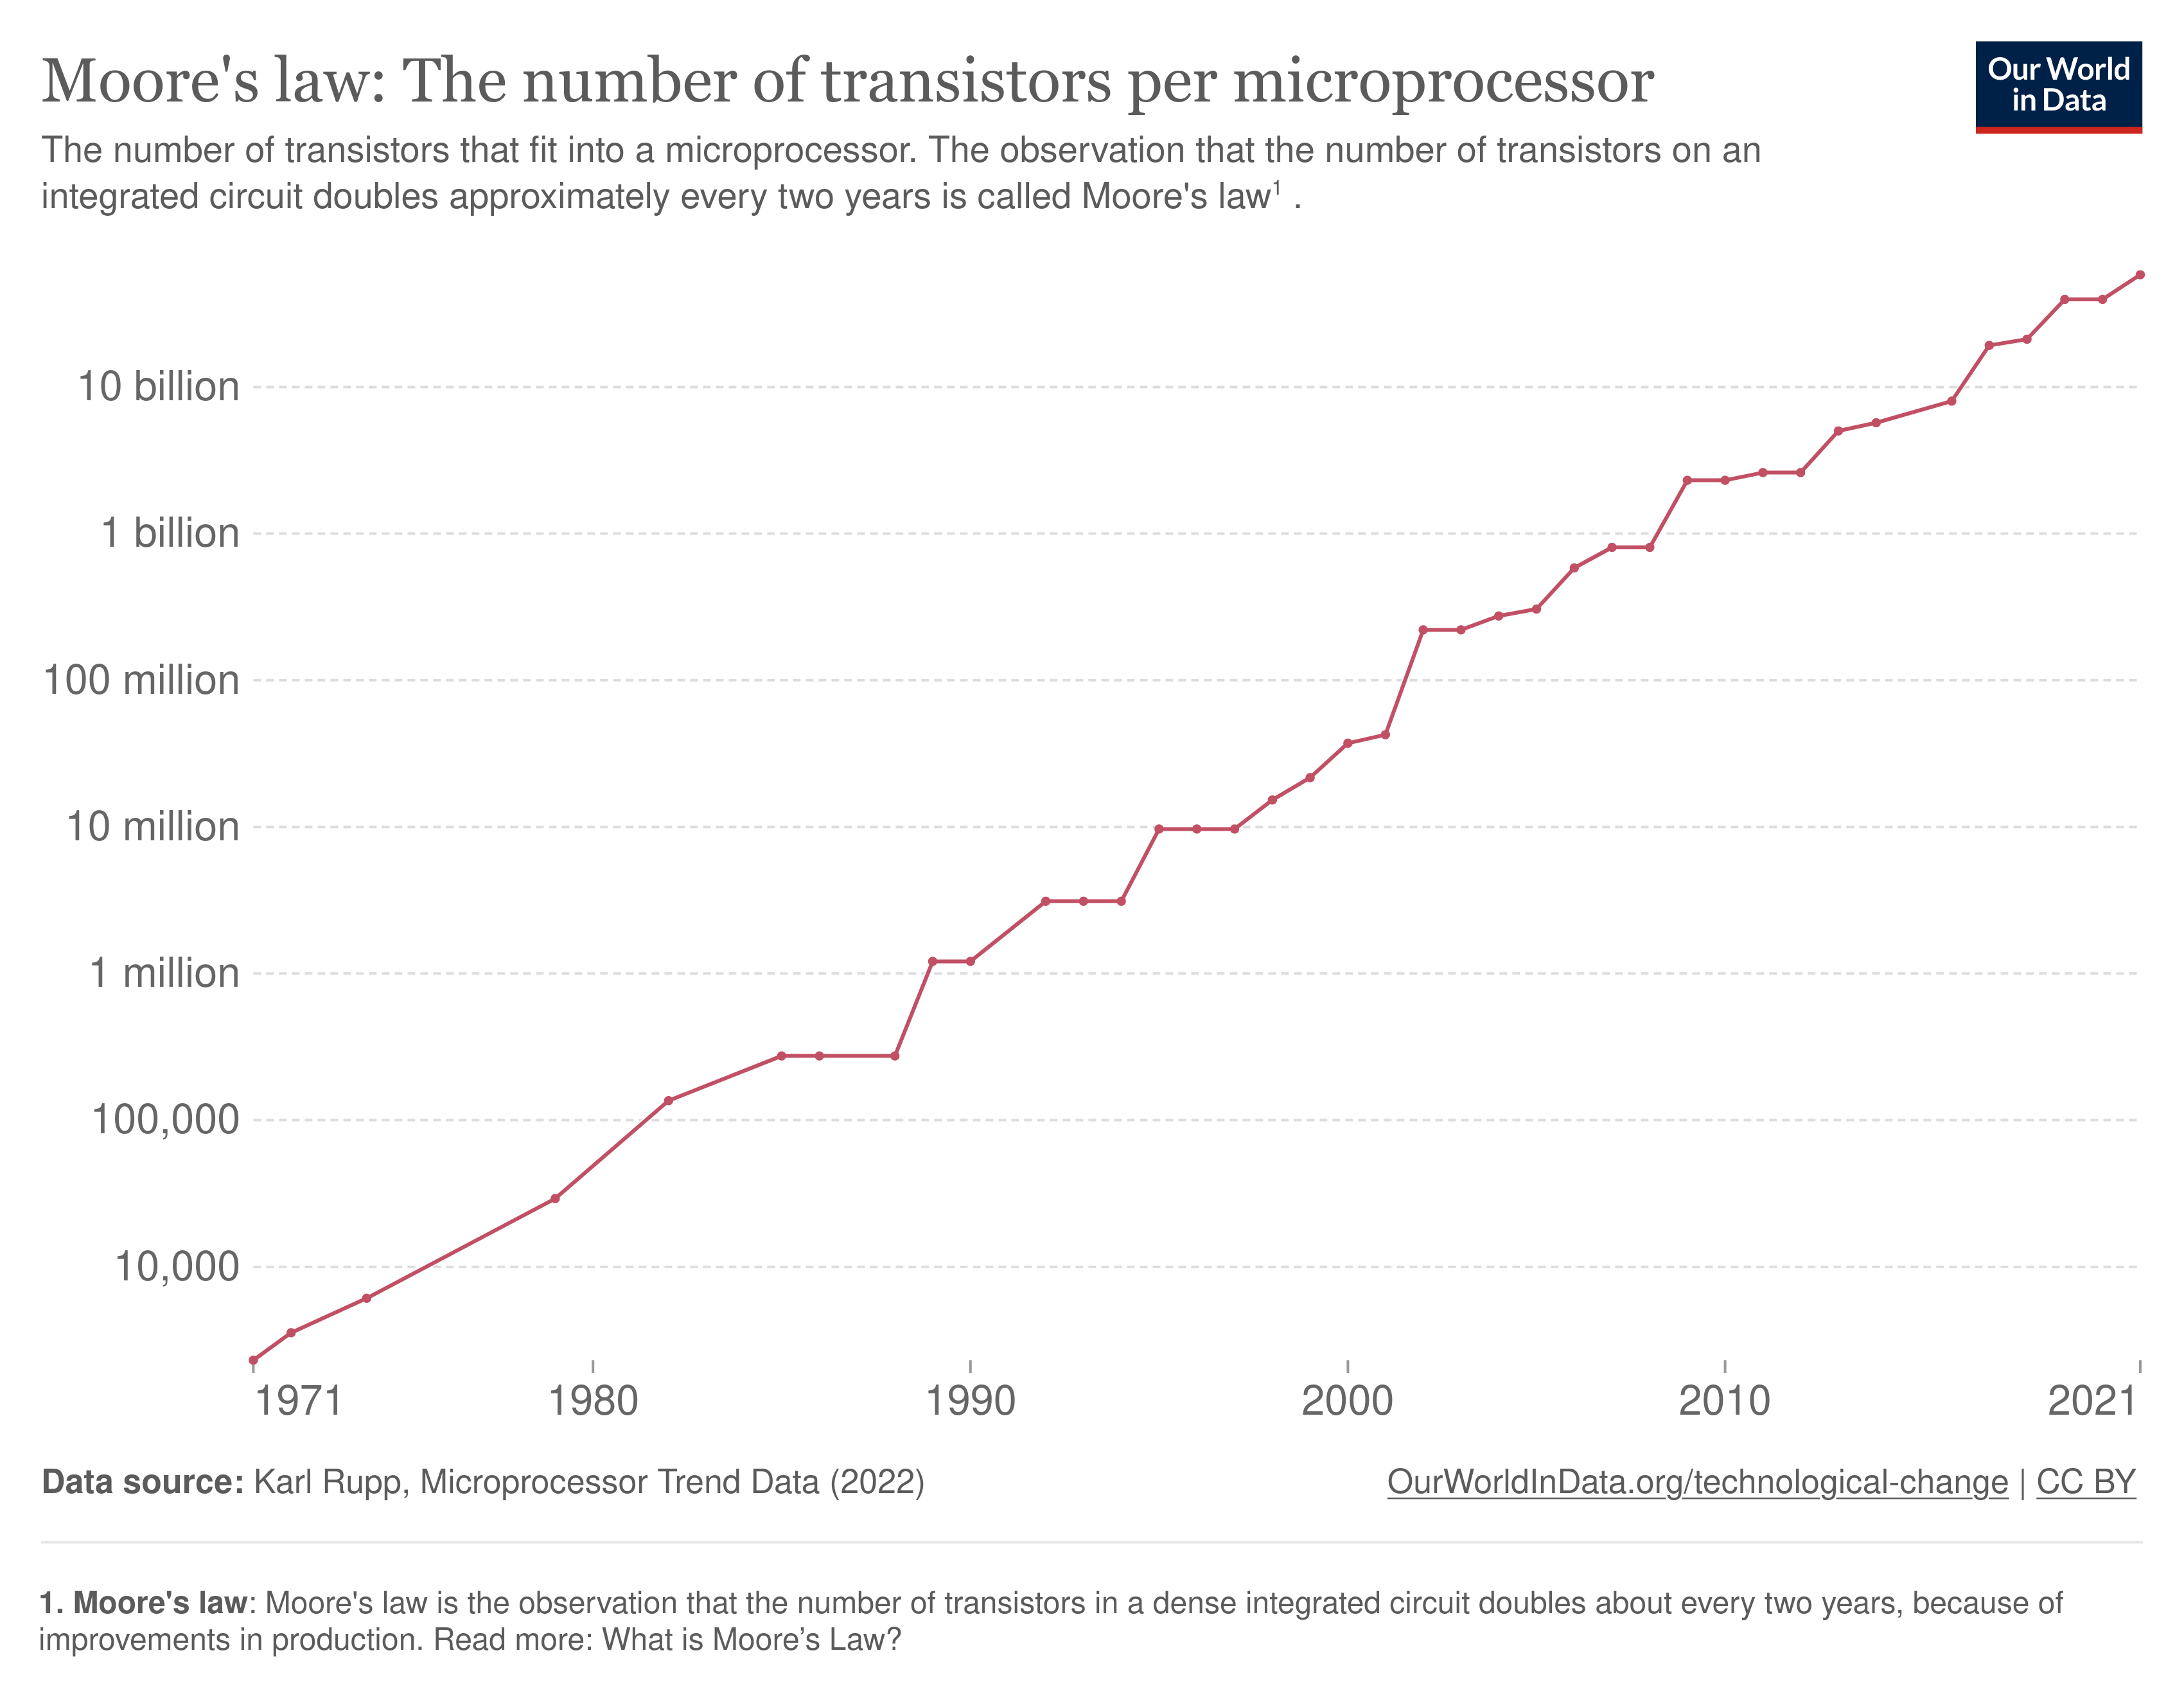
\includegraphics[width=.9\linewidth]{images/chapter1/moore_law2.png}
\caption{Legge di Moore}
\label{fig:moore_law}
\end{figure}

% GPU

Le \gls{GPU} sono hardware specializzato che prende a piene mani il concetto di multi-core e lo esalta, al punto da avere tantissimi core più semplici e lenti dei core di una CPU, ma con un più alto throughput totale. 
Originariamente sono state sviluppate per scopi legati all'elaborazione grafica, in particolare, per migliorare la resa delle immagini e la grafica 3D nei videogiochi, nelle applicazioni \gls{CAD} e nei software di modellazione e renderin. In seguito, le esigenze di una grafica sempre più dettagliata e complessa ha portato alla creazione di unità di elaborazione specializzate con un'architettura che le rende energicamente più efficienti di una CPU per algoritmi che processano grossi blocchi di dati in parallelo. Le GPU sono state quindi fruttate, anche per scopi diversi dall'elaborazione grafica e si sono rivelate particolamenti utili per applicazioni scientifiche, \gls{HPC} e tecniche che richiedono elaborazione intensive, come la simulazione, l'analisi dei dati e il calcolo scientifico. Adesso in particolare le GPU si sono particolarmente adatte per l'addestramento e l'implementazione di reti neurali, diventando uno strumento fondamentale per l'esplosione dell'intelligenza atrificiale e del machine learning.

% GPGPU

Quando si parla di \gls{GPGPU} si intende l'utilizzo delle GPU per compiti di calcolo generale, per renderle molto più che semplici dispositivi per l'elaborazione grafica. Questo è fondamentale per accelerare algoritmi di calcolo che richiedono enorme quantità di risorse, a patto che la computazione sia parallelizzabile su più processori.
Calcoli che prima richiedevano l'uso di supercomputer, per essere eseguiti, adesso si possono eseguire con una normale GPU desktop. 
Nel 2011 secondo la lista Top500, che classifica e descrive nel dettaglio i 500 sistemi informatici non distribuiti più potenti al mondo, il Tianhe-1A risultava il secondo supercomputer più potente al mondo, raggiungendo i 4.7 petaFLOPS di potenza computazionale, grazie a un sistema basasto sulle GPU Nvidia Tesla M2050 \cite[]{Tianhe-1A:link}. Solamente un anno dopo, invece, in in vetta alla classifica si trovò il Titan \cite[]{Titan:link} con un sistema basato sulle più recenti e performanti GPU Nvida Tesla K20X raggiungendo i 17.59 petaFLOPS di potenza.
Da quell'anno in poi divenne chiaro che le GPU erano diventate un componente essenziale nell'HPC tanto quanto lo erano nel desktop computing e dato che il supercomputing è il motore trainante di molte delle tecnologie che vediamo nei processori moderni, si è venuto a creare un circolo virtuoso per cui la necessità di processori sempre più veloci per elaborare dataset sempre più grandi, ha porta l'industria a produrre computer sempre più potenti. Ad oggi si sta delineando una divisione netta nella produzione di GPU per uso desktop e per uso scientifico, i principali produttori, quali AMD, Nvidia e, più recentemente, Intel, rilasciano prodotti ottimizzati per l'uno o per l'altro mercato, con lo scopo di soddisfare i requisiti richiesti da ogni settore. A giugno 2023 il supercomputer più veloce al mondo è il Frontier \cite[]{Frontier:link} con un sistema basato sulle GPU Radeon Instinct MI250X con coi riesce a raggiungere i 1.67 exaFLOPS, divenendo il primo exacale supercomputer al mondo. L'incremento così repentino delle performance ha portato gli esperti di settore a coniare (?) la legge di Huang \cite[]{Huang:law}, per cui le performance delle GPU più che raddoppiano ogni due anni. In pratica un'equivalente della di Moore, ma applicata alle GPU.

\begin{figure}[ht]
\centering
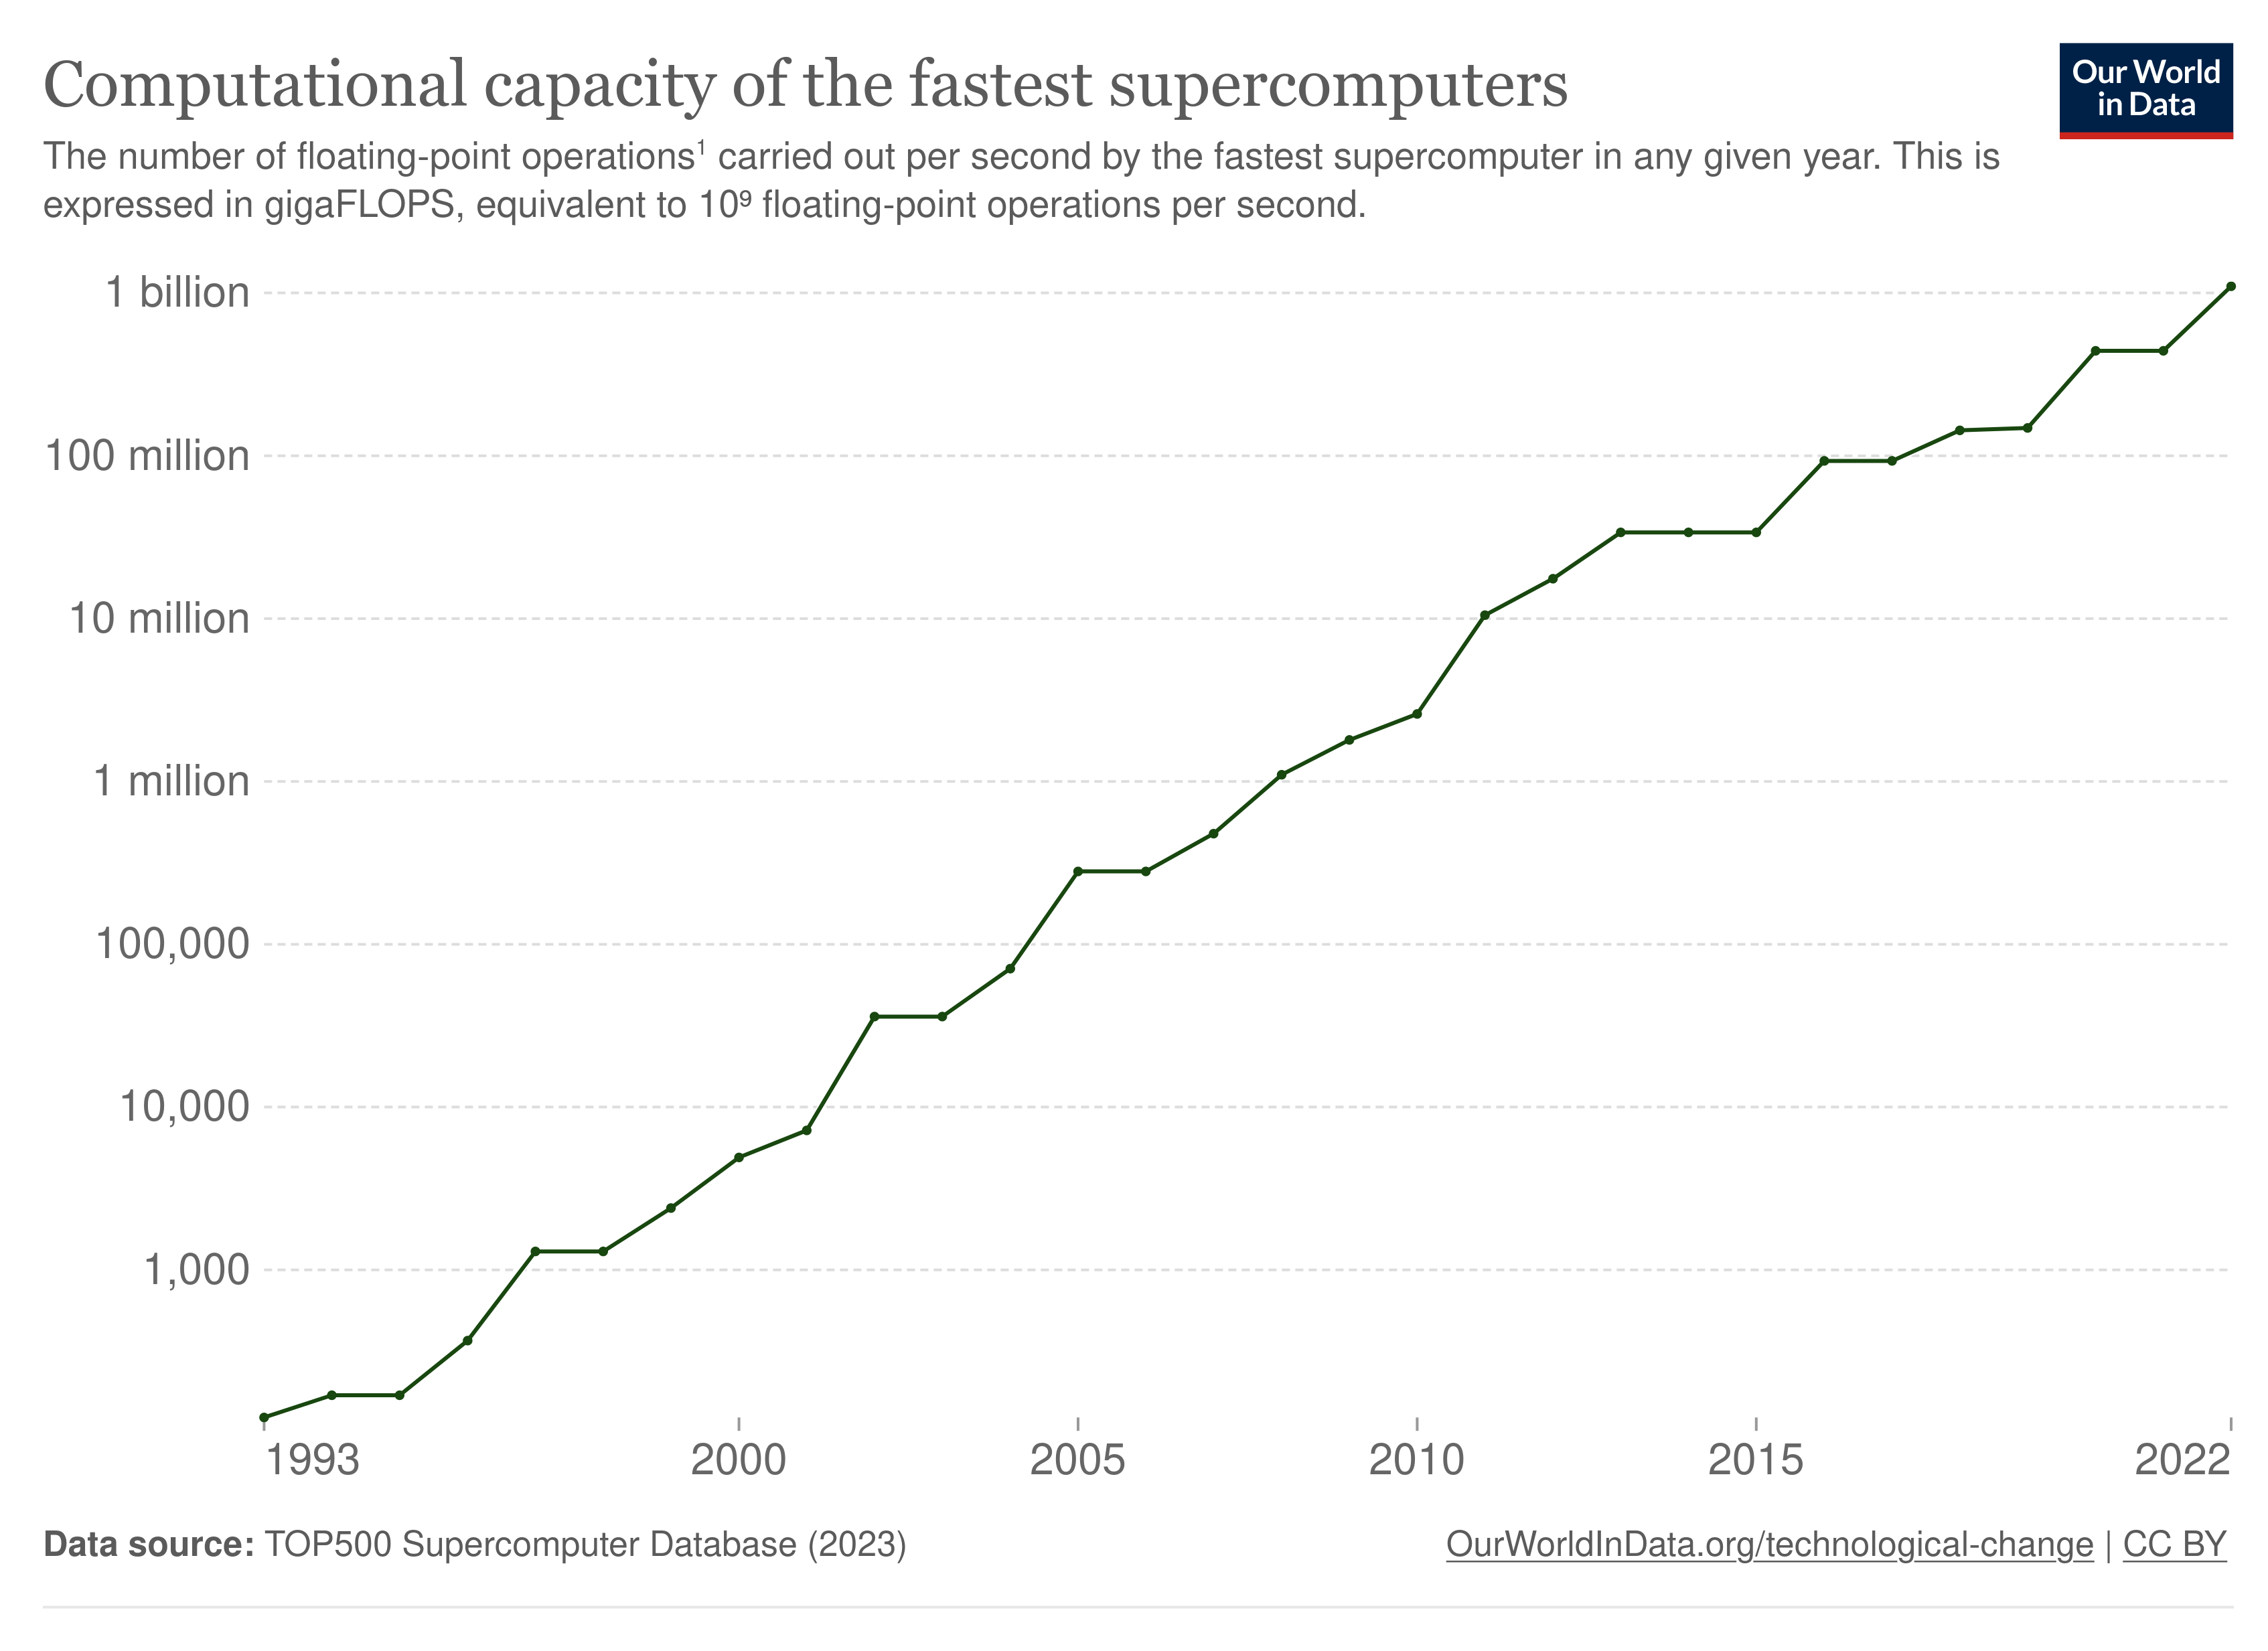
\includegraphics[width=.9\linewidth]{images/chapter1/supercomputer_flops.png}
\caption{Potenza dei supercomputer negli anni}
\label{fig:supercomputer_flops}
\end{figure}
    
%% Librerie GPU programming

Per poter programmare le GPU è risutanto necessario sviluppare delle \gls{API} che garantissero l'esecuzione del programma senza un'esplicita conversione dai dati in formato grafico. Le API oggi più utilizzate sono le \gls{CUDA} API di Nvidia \cite[]{Nvidia:CUDA} e le OpenCL API di Khronos Group \cite[]{KG:OpenCL}. Le API CUDA sfruttano l'omonima architettura delle GPU Nvidia e sono in formato proprietario, mentre le API OpenCL, come suggerisce il nome, sono uno standard aperto royalty-free e supportano la maggior parte delle archittetture GPU. Sebbene avesse prestazioni di molto inferiori rispetto a CUDA, OpenCL è storicamente stata la prima scelta per applicazioni multi-piattaforma, proprio per la sua natura open e la vasta quantità di hardware supportato. Nel 2015 Khronos Group annuncia le Vulkan API \cite[]{KG:Vulkan} e SPIR-V \cite[]{KG:SPIR-V}. Vulkan è una API grafica e di calcolo che offre un accesso ad alta efficienza e multi-piattaforma alle GPU moderne utilizzate in una vasta gamma di dispositivi, da PC e console ai telefoni cellulari e alle piattaforme embedded. Vulkan è stato progettato per sfruttare pesantemente il multithreading, permettendo la generazione di carichi di lavoro asincroni da parte di thread mulitpli della CPU che eseguono il codice sulla GPU solo dopo una esplicita sottomissione. Inoltre, la sua natura `close-to-metal' permette un controllo oculato delle risorse della GPU: lo sviluppatore è resposabile della sincronizzazione, allocazione di memoria e della sottomissione del lavoro, avendo così minor overhead del driver rispetto ad approcci come CUDA e OpenCL.

\section[Problema e Contributi]{Problema e Contributi}


L'elaborato si pone come obiettivo quello di trovare e valutare possibili vantaggi nello sviluppare un'applicazione di computing in Vulkan e Rust, per un ambiente a microservizi, rispetto a CUDA.
Nonostante Vulkan sia largamente usato nell'industria dei videogiochi, usarlo in ambito computing è una sfida non banale, a causa delle API verbose e del controllo meticoloso delle strutture dati. 
Un'idea per ridurre il carico intellettivo per lo sviluppatore, e rendere la develpement experience meno gravosa, può essere quella di consentire gestione della memoria in modo automatico, pur manetendo prestazioni quanto più vicine possibili a un'implementazione ``low level'', per questo motivo si è coniugato i vantaggi del linguaggio Rust con quelli che offre Vulkan. 

Per poter capire se Vulkan con Rust è una valida alternativa a CUDA per il computing bisogna rispondere alle seguenti domande:

% bullet points
\begin{itemize}
    \item Qual è il livello di performance che Vulkan riesce a raggiungere rispetto a CUDA? 
    \item Quanto è difficile sviluppare un'applicazione per il computing in Vulkan?
    \item In un ambiente a microservizi, quanto è facile sviluppare e mantenere un'applicazione Vulkan scritta in Rust? 
    \item Qual è il livello di maturità dell'ecosisistema Vulkan e quello di Rust?
\end{itemize}

Si è provato a rispondere a queste domande nel senguente modo:

\begin{itemize}
    \item Si è scelto di implementare algoritmi altamente parallelizzabili su GPU, quali la somma di vettori e moltiplicazione di matrici, da usare come banco di prova per comparare le performance di due medesime implementazioni in CUDA e Vulkan, in particolare è preso in considerazione sia il tempo dell'esecuzione ``pura'' dell'algoritmo, che del trasferimento dei dati dalla memoria host (CPU) a quella device (GPU).
    \item Si è implementato gli algoritmi in Vulkan per valutare il potenziale delle sue API close-to-metal e quanto ergonomico sia sviluppare mediante Rust. Dato che sviluppare in Vulkan richiede degli step standard quali la creazione di un logical device, una pipeline, la lettura del codice kernel e l'allocazione di memoria, si è usata la libreria Rust Vulkano \cite[]{github:Vulkano}, che implementa dei binding safe all'implementazione standard di Vulkan.
    \item Si è poi reimplementato i medesimi algoritmi in CUDA per comparare sia le performance che il diverso approccio alla scrittura dei kernel come estensione del linguaggio C++ tramite il compilatore nvcc \cite[]{Nvidia:nvcc}, osservando che GLSL \cite[]{KG:GLSL} usato in Vulkan offre più ottimizzazioni orientati alla grafica che al computing.
    \item Infine, considerando le necessità aziendali e i risultati relativi ai benchmark ottenuti, si è sviluppato un microservizio proof of concept che conuigare i vantaggi di Rust in ambito web e quelli di CUDA in ambito computing, valutando anche altri approcci nella soluzione del problema.
\end{itemize}



\section[Struttura della tesi]{Struttura della tesi}

!! TODO quando finiti tutti i capitoli

Il lavoro è stato progettato, sviluppato e testato con il supporto del team di Quantum Computing di Data Reply con sede a Torino. 



\paginavuota
\ringraziamenti % acknowledgements
% acknowledgements


Ogni viaggio inizia con un primo passo, e oggi posso dire di aver compiuto un passo importante. Guardo indietro e vedo il lungo sentiero che ho percorso per arrivare fin qui, un cammino troppo insidioso da intraprendere senza il sostegno delle persone che mi sono state vicine, condividendo con me difficoltà e gioie. Vorrei esprimere la mia profonda gratitudine a tutte queste persone, i cui contributi hanno reso possibile il raggiungimento di questo grande traguardo.

Un grazie di cuore va al Prof.~Giovanni Malnati, relatore di questa tesi, per avermi guidato e supportato in questo percorso, per avermi dato la possibilità di esplorare nuovi orizzonti e per avermi trasmesso la passione per la ricerca, l'innovazione e soprattutto per Rust. Grazie per avermi dato la possibilità di lavorare a questo progetto.

Un doveroso ringraziamento va ai miei azionisti di maggioranza, senza i quali tutto questo non sarebbe stato possibile: Madre e Padre. Supporto finanziario ed emotivo che mi ha permesso di iniziare e concludere (quasi incolume) questo viaggio.

A Sorella, che, dalle tagliatelle con la salsa cruda ai pastel de Nata, è stata il supporto calorico e caloroso di cui avevo bisogno, ``sem queijo, sem leite''.

Alla famiglia di giù, che ha deciso di spargersi per l'Italia: ``scendere per le feste'' è di per sè una festa solo perché ci siete tutti voi.

Alla famiglia che ho trovato su e mi ha fatto sentire a casa, sopravvivendo a tutti i miei drammi e dad joke: grazie per essere stati compagni insostituibili di questo viaggio. Che fosse una pampanella, un frico, una carbonara, una fregola, una pasta zucchine e Philadelphia, un sushi, una genziana o semplicemente un caffè, quei momenti passati insieme hanno reso meno gravosa questa scalata, che in solitaria sarebbe stata insostenibile.

Agli altri due moschettieri che da 20 anni mi supportano e sopportano: ce l'abbiamo fatta, adesso siamo un trio di dottori.

A voi tutti un grazie dal più profondo del mio cuore, mi avete fatto capire perché ``amicizia'' ha la stessa radice di ``amore''.

Al team Policumbent e soprattutto ai nevadini: abbiamo condiviso sia esperienze fantastiche che momenti terrificanti. Ogni istante lo custodirò gelosamente e rimarrò per sempre legato a all'avventura che abbiamo intrapreso insieme. Bikes on the road!

Voglio dedicare questo lavoro di tesi, e tutto il percorso che oggi si conclude, alla persona che per prima in assoluto ha creduto in me (anche se mi avrebbe voluto avvocato). Nonna Pina, so che non potrai leggere o sentire queste parole, ma sarai l'unica ad avere il nome tra queste pagine. In qualsiasi tempo e luogo tu sia, spero possa arrivarti chiaro che ``nasca bedda'' si è appena laureato ingegnere.

Concludo lasciando un messaggio al me futuro, che sicuramente col tempo rileggerà queste parole: ``lo so, la salita è stata dura e da qui la vista è meravigliosa, ma non non è finita. Questo non è che il primo campo base, la cima è lassù che ci aspetta e io ho già la bandiera in mano''.


% actually abbreviation is the name used for acronym in glossaries-extra
% title sets the name
% type tells the type of glossary to print
% style overrides the global style
% here we are printing only abbreviations
% printunsrtglossary if using record, otherwise printglossary is ok
\paginavuota
\printunsrtglossary[style=altlist,title=Glossario,type=\glsxtrabbrvtype]


% \paginavuota % it works even without stile=classica

% \appendix
% % appendix
\chapter{Galileo}
\label{sec:appendix_galileo}

%\lstinputlisting[]{} % for source code files directly
% lstlisting environment for direct inclusion
\begin{lstlisting}[language=Python]
    import os
    os.system("echo 1")
\end{lstlisting}

% for computational complexity
$\mathcal{O}\left(n\log{n}\right)$

% verbatim
\verb+numpy+



% endnotes here if needed

\phantom{0}
\cleardoublepage
\printbibliography[heading=bibintoc] % heading required to show it in ToC

\end{document}
